% !TeX root = ../main.tex
\chapter{BẢNG KÊ NHIỆM VỤ VÀ ĐÁNH GIÁ}
\section{Bảng kê nhiệm vụ}
Bảng dưới kế thừa phân công đang lưu trong hồ sơ nhóm. Mỗi hàng chỉ đánh dấu một người phụ trách chính; nội dung tích hợp có thể được kiểm tra chéo. Các cột dùng bốn số cuối MSSV để tránh thu hẹp cột mô tả. Tỉ lệ đóng góp là mức đề xuất, không phải điểm đã được giảng viên xác nhận.
\begin{table}[H]\small\centering\caption{Danh sách thành viên và tỷ lệ điểm đề xuất}
\begin{tabularx}{\linewidth}{@{}lYc@{}}\toprule\textbf{MSSV}&\textbf{Họ và tên}&\textbf{Đề xuất}\\\midrule
2410709&Nguyễn Thành Đạt&20\%\\2410694&Nguyễn Minh Đạt&20\%\\2410696&Nguyễn Phúc Bảo Đạt&20\%\\2413095&Nguyễn Hữu Tây&20\%\\2413181&Trần Tiến Thành&20\%\\\bottomrule\end{tabularx}\end{table}
\begingroup\small\setlength{\tabcolsep}{3pt}\renewcommand{\arraystretch}{1.15}
\begin{longtable}{@{}>{\raggedright\arraybackslash}p{82mm}ccccc@{}}\caption{Bảng kê người phụ trách từng nội dung}\\\toprule
\textbf{Nội dung} &\textbf{0694}&\textbf{0696}&\textbf{3095}&\textbf{0709}&\textbf{3181}\\\midrule\endfirsthead
\toprule\textbf{Nội dung (tiếp)} &\textbf{0694}&\textbf{0696}&\textbf{3095}&\textbf{0709}&\textbf{3181}\\\midrule\endhead
\bottomrule\endfoot
Tạo bảng dữ liệu phần 1: 12 bảng danh tính và máy trạm & x &  &  &  & \\
Tạo bảng dữ liệu phần 2: 11 bảng dịch vụ, kho, ca trực và ví &  &  & x &  & \\
Tạo các ràng buộc khóa chính, duy nhất và miền giá trị (CHECK) & x &  &  &  & \\
Tạo các ràng buộc khóa ngoại bảo toàn toàn vẹn tham chiếu &  &  & x &  & \\
Demo kiểm tra tạo bảng, ràng buộc và kiểm đếm 23 bảng thành công & x &  &  &  & \\
Tạo chỉ mục phần 1: ix\_dich\_vu\_filter tăng tốc lọc thực đơn &  &  &  &  & x\\
Tạo chỉ mục phần 2 cho các bảng vận hành &  & x &  &  & \\
Đo lường hiệu năng chỉ mục trước và sau bằng EXPLAIN ANALYZE &  &  &  &  & x\\
Câu truy vấn 1 (Q-P12-01) - Bảng liên quan: MAY\_TRAM, KHU\_VUC & x &  &  &  & \\
Câu truy vấn 2 (Q-P12-02) - Bảng liên quan: DICH\_VU, NHOM\_DICH\_VU &  & x &  &  & \\
Câu truy vấn 3 (Q-P12-03) - Bảng liên quan: DON\_GOI\_DICH\_VU &  & x &  &  & \\
Câu truy vấn 4 (Q-P12-04) - Bảng liên quan: CA\_TRUC, PHAN\_CONG\_TRUC &  &  &  &  & x\\
Câu truy vấn 5 (Q-P12-05) - Bảng liên quan: NGUOI\_CHOI, GIAO\_DICH\_VI &  &  & x &  & \\
Thủ tục INSERT (sp\_khu\_vuc\_insert) - Bảng: KHU\_VUC & x &  &  &  & \\
Thủ tục UPDATE (sp\_khu\_vuc\_update) - Bảng: KHU\_VUC & x &  &  &  & \\
Thủ tục DELETE (sp\_khu\_vuc\_delete) - Bảng: KHU\_VUC & x &  &  &  & \\
Demo kiểm tra ba thủ tục CRUD khu vực với các ca đúng và lỗi & x &  &  &  & \\
Trigger 1 (T-P12-01) - Bảng: BIEN\_LAI\_TIEN\_MAY &  &  & x &  & \\
Demo kiểm tra Trigger 1 chặn sửa/xóa biên lai đã thanh toán &  &  & x &  & \\
Trigger 2 (T-P12-02) - Bảng: CHI\_TIET\_GOI\_DICH\_VU, DON\_GOI\_DICH\_VU &  &  &  & x & \\
Demo kiểm tra Trigger 2 duy trì tổng tiền đầu đơn từ chi tiết &  &  &  & x & \\
Thủ tục 1 (sp\_bao\_cao\_doanh\_thu\_ngay) - Bảng: BIEN\_LAI, DON\_GOI &  & x &  &  & \\
Demo kiểm tra Thủ tục 1 tổng hợp doanh thu theo ngày &  & x &  &  & \\
Thủ tục 2 (sp\_bao\_cao\_ton\_dich\_vu) - Bảng: DICH\_VU, NHOM\_DICH\_VU &  &  &  &  & x\\
Demo kiểm tra Thủ tục 2 phân loại tồn kho bằng CURSOR và IF &  &  &  &  & x\\
Hàm 1 (fn\_tong\_chi\_vi\_rong) - Bảng: GIAO\_DICH\_VI, NGUOI\_CHOI &  &  & x &  & \\
Demo kiểm tra Hàm 1 tính tổng chi ví ròng &  &  & x &  & \\
Hàm 2 (fn\_tong\_tien\_don) - Bảng: CHI\_TIET\_GOI\_DICH\_VU &  &  &  & x & \\
Demo kiểm tra Hàm 2 tính tổng tiền đơn hàng &  &  &  & x & \\
Kiến trúc tích hợp Backend Flask và Test suite tự động 79 ca &  &  &  & x & \\
Thiết kế sơ đồ giải thuật lưu đồ TikZ cho toàn bộ Routine & x &  &  &  & \\
Kịch bản dữ liệu và benchmark đo lường chỉ mục &  & x &  &  & \\
\end{longtable}\endgroup
\clearpage\section{Đánh giá của giáo viên}
(Điền danh sách thành viên và \% đóng góp bên dưới và để trống các cột còn lại)
\begin{table}[H]\centering\small\renewcommand{\arraystretch}{2.2}
\begin{tabularx}{\linewidth}{@{}>{\raggedright\arraybackslash}p{36mm}lp{12mm}Y>{\raggedright\arraybackslash}p{13mm}p{13mm}@{}}\toprule
\textbf{Họ tên}&\textbf{MSSV}&\textbf{Đề xuất}&\textbf{Nhận xét}&\textbf{Điểm trừ/cộng}&\textbf{Tổng}\\\midrule
Nguyễn Thành Đạt&2410709&20\%&&&\\
Nguyễn Minh Đạt&2410694&20\%&&&\\
Nguyễn Phúc Bảo Đạt&2410696&20\%&&&\\
Nguyễn Hữu Tây&2413095&20\%&&&\\
Trần Tiến Thành&2413181&20\%&&&\\\bottomrule
\end{tabularx}\end{table}
\chapter{PHỤ LỤC: Thiết kế ERD cập nhật mới nhất}\label{app:eer}
\section{Sơ đồ tổng thể EER dạng vector}
Sơ đồ tuân thủ chặt chẽ ký hiệu Chen chuẩn (thực thể hình chữ nhật, mối quan hệ hình thoi, thuộc tính hình elip, khóa chính gạch chân, thực thể và liên kết yếu nét đôi, thuộc tính đa trị nét đôi, thuộc tính dẫn xuất nét đứt, tham gia toàn phần nét đôi), được đồng bộ lại theo phong cách đơn sắc đen trắng rõ nét. Sơ đồ bao quát toàn bộ 18 thực thể và tất cả các mối quan hệ nghiệp vụ của hệ thống 23 bảng. Tệp PDF/SVG nguồn vector được lưu tại \path{assets/eer/erd_full_vector.pdf} và mô hình chỉnh sửa tại \path{docs/btl1_baseline/BTL1_EER.drawio}.
\begin{figure}[H]\centering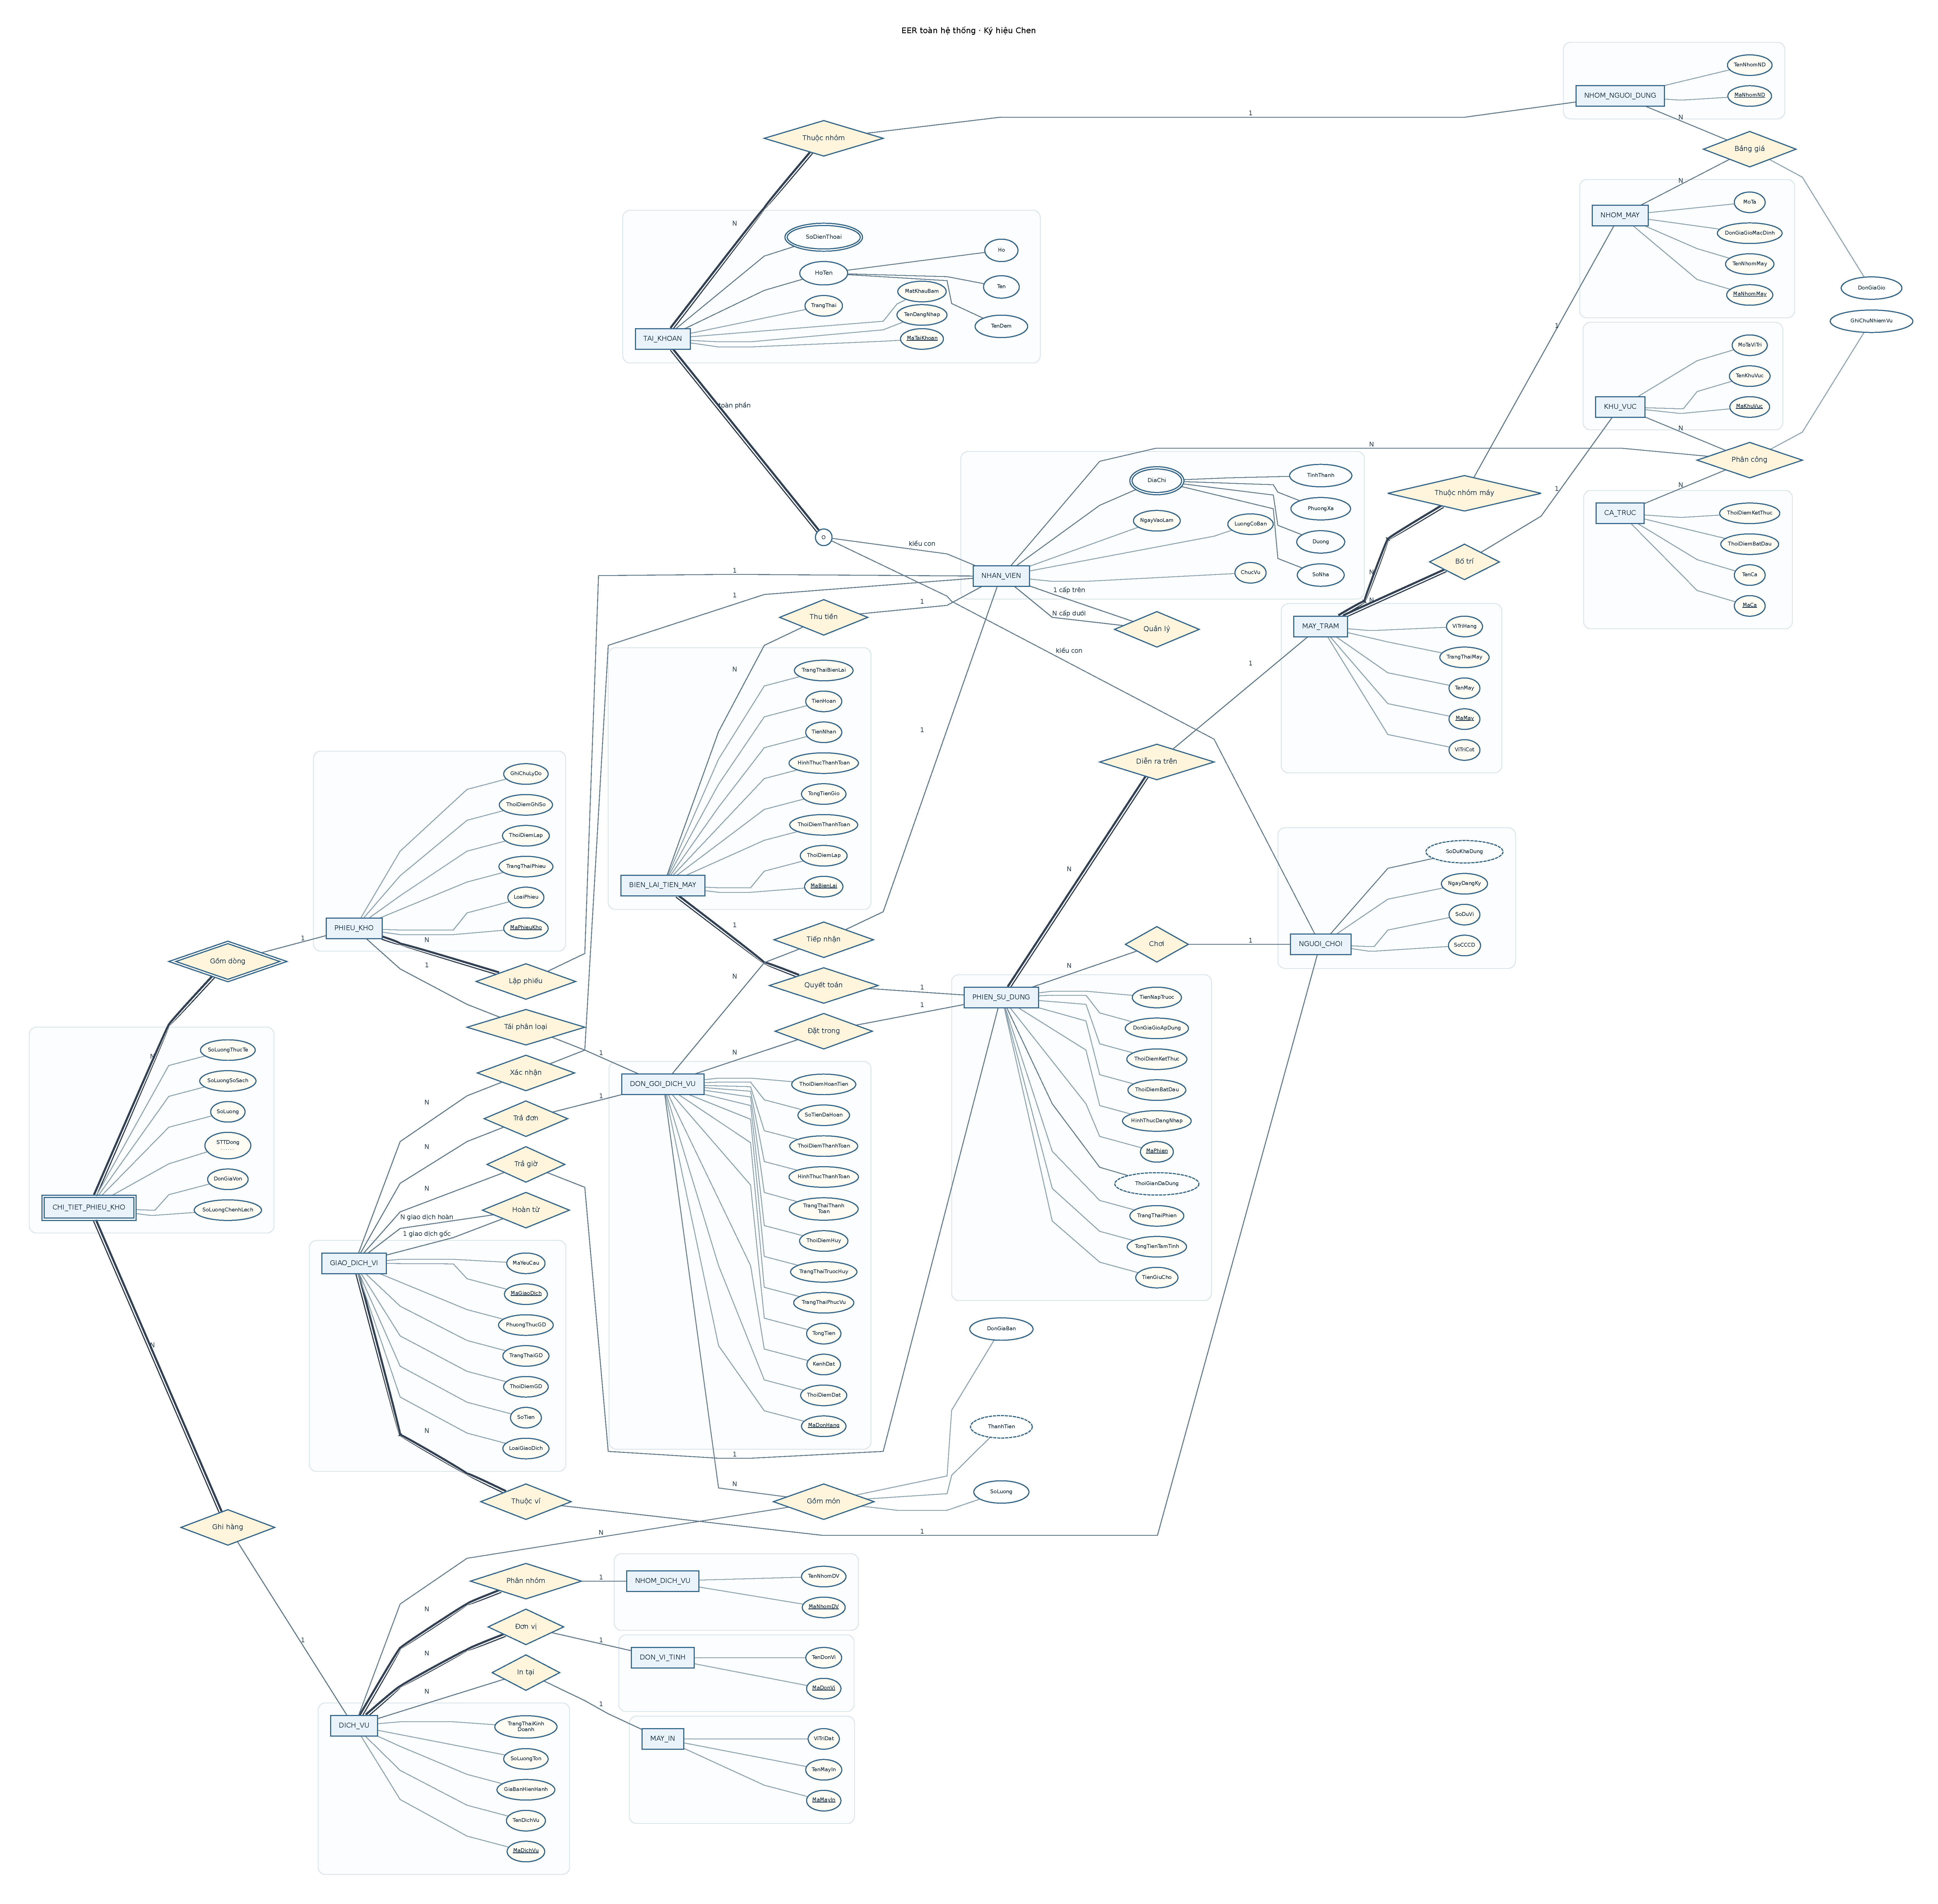
\includegraphics[width=\linewidth,height=.82\textheight,keepaspectratio]{assets/eer/erd_full_vector.pdf}\caption{Sơ đồ EER tổng thể toàn hệ thống theo ký hiệu Chen}\end{figure}
\clearpage\section{Bảng ghi chú các thay đổi so với BTL1}
\begingroup\small\setlength{\tabcolsep}{3.5pt}\renewcommand{\arraystretch}{1.2}
\begin{longtable}{@{}>{\raggedright\arraybackslash}p{28mm}>{\raggedright\arraybackslash}p{38mm}>{\raggedright\arraybackslash}p{44mm}>{\raggedright\arraybackslash}p{44mm}@{}}\toprule
\textbf{Nội dung thay đổi}&\textbf{Phiên bản cũ (BTL1)}&\textbf{Phiên bản mới (BTL2)}&\textbf{Lí do}\\\midrule\endhead
\bottomrule\endfoot
Duy nhất có điều kiện&Chỉ có ràng buộc quan hệ thực thể, chưa ràng buộc mức DBMS chống phiên mở đồng thời.&Bổ sung cột sinh và chỉ mục UNIQUE có điều kiện cho phiên đang hoạt động.&Ngăn chặn triệt để 1 tài khoản mở nhiều phiên hoặc 1 máy trạm mở cùng lúc 2 phiên.\\\midrule
Đồng bộ tổng tiền đơn&Tổng tiền đơn tính độc lập hoặc dựa vào logic tầng ứng dụng.&Bộ 3 AFTER trigger trên chi tiết dịch vụ tự động đồng bộ lại tổng tiền đầu đơn.&Bảo toàn tính nhất quán dữ liệu kế toán, không phụ thuộc ứng dụng ngoài.\\\midrule
Phân định ngày doanh thu&Thống kê doanh thu theo ngày tạo đơn hoặc ngày tạo phiên.&Tách riêng thời điểm thanh toán biên lai/đơn và thời điểm hoàn tiền.&Phản ánh đúng dòng tiền thực tế theo ngày phát sinh thay vì ngày đặt đơn.\\\midrule
Miền giá trị tiền tệ trong hàm&Dùng INT hoặc DECIMAL ngắn trong các biến tính toán của hàm.&Chuẩn hóa sang DECIMAL(18,0) cho toàn bộ biến tổng và kết quả trả về của hàm.&Tránh tràn số và sai lệch số học khi tổng tiền hoặc giao dịch ví quy mô lớn.\\\midrule
Miền chuỗi Cursor trong thủ tục&Khai báo biến tạm VARCHAR(50) ngắn trong thân thủ tục.&Khai báo khớp độ dài lược đồ (VARCHAR(100) cho tên, VARCHAR(30) cho đơn vị).&Tránh lỗi cắt cụt chuỗi dữ liệu (Data truncation) khi duyệt báo cáo tồn kho.\\\midrule
Tối ưu hóa chỉ mục thực đơn&Chỉ có các khóa chính và khóa ngoại mặc định theo thiết kế ERD.&Tạo chỉ mục phức hợp \texttt{ix\_dich\_vu\_filter} trên \texttt{(trang\_thai, ma\_nhom, ten\_dich\_vu)}.&Giảm chi phí đọc và tăng tốc truy vấn lọc thực đơn 3.88x (đo bằng EXPLAIN ANALYZE).\\\bottomrule
\end{longtable}\endgroup
\chapter{Dữ liệu mẫu và nguồn minh chứng}\label{app:data}
Mỗi hình dưới là bản xuất của SQL client trong cùng phiên kiểm chứng với các truy vấn ở Phần 1. Các dữ liệu là dữ liệu demo; không sử dụng thông tin cá nhân thật. Phần SQL và kết quả thô đầy đủ đi kèm ở thư mục evidence/dbms.
\snapshot{q01_data}{Các bảng dữ liệu mẫu liên quan Q-P12-01}{fig:q01_data}
\snapshot{q02_data}{Các bảng dữ liệu mẫu liên quan Q-P12-02}{fig:q02_data}
\snapshot{q03_data}{Các bảng dữ liệu mẫu liên quan Q-P12-03}{fig:q03_data}
\snapshot{q04_data}{Các bảng dữ liệu mẫu liên quan Q-P12-04}{fig:q04_data}
\snapshot{q05_data}{Các bảng dữ liệu mẫu liên quan Q-P12-05}{fig:q05_data}
\section{Nguồn và khả năng tái tạo}
\begin{itemize}
\item Đề gốc và mẫu Updated: thư mục \path{docs/requirements/} và tệp mẫu trong \path{docs/} của gói bàn giao.
\item DDL, khóa và routine: \path{database/01_schema/} đến \path{database/08_triggers/}.
\item Minh chứng trực tiếp: \path{evidence/dbms/manifest.json}; mỗi mục ánh xạ ảnh, câu SQL và kết quả JSON.
\item Số đo chỉ mục: \path{evidence/queries/index_benchmark.json}; kiểm thử: \path{evidence/final_verification/}.
\item Nguồn sơ đồ EER: \path{docs/btl1_baseline/BTL1_EER.drawio}; các bản vector dùng trong báo cáo nằm tại \path{assets/eer/} của bộ LaTeX.
\item Nguồn báo cáo: \path{main.tex}, các tệp \path{sections/}, \path{diagrams/} và \path{sql/}. Biên dịch bằng XeLaTeX để giữ nguyên tiếng Việt và phông chữ.
\end{itemize}
